\section{Introduzione all'astrofisica osservativa}\label{sec:astrofisica-osservativa}
Come introdotto nel paragrafo~\ref{sec:introduzione}, l'astrofisica studia le strutture cosmiche in maniera indiretta attraverso la radiazione che raccogliamo con i telescopi e altri strumenti. In particolare, osservando a bande diverse, si possono estrapolare informazioni quantitative dalla misura della radiazione. Si tenga tuttavia a mente che la radiazione che riceviamo dipende sia dai processi fisici che l'hanno generata sia da quelli che ha subito nel tragitto tra la sorgente e l'osservatore.

Il primo problema dell'osservazione è il così detto \emph{assorbimento atmosferico}. Infatti, non tutta la radiazione emessa dagli oggetti astrofisici riesce a raggiungere la superficie terrestre. In particolare, ci giungono il vicino ultravioletto, il vicino infrarosso e le onde radio e visibili, mentre il resto della radiazione non arriva a terra perché viene assorbita dall'atmosfera. È dunque necessario osservare con telescopi spaziali in orbita. Un altro problema che si riscontra è quello del \emph{seeing}, secondo il quale le particelle di vapor acqueo dell'atmosfera creano una turbolenza che sfoca le immagini acquisite dai telescopi. Per questo motivo è conveniente effettuare le osservazioni in posti poco umidi, come il Cile o le Hawaii. Senza tecniche per correggere tale problema sarebbe inutile cercare di avere telescopi di diametro maggiore per avere una maggior qualità dell'immagine. Guardando una stella, generalmente l'immagine risulta un disco sulla lente, mentre se c'è turbolenza si ha un'immagine distorta e che si muove. Un'immagine affetta dal problema del seeing si dice \emph{seeing-limited}. Si chiama inoltre \emph{diffraction-limited} la minore distanza angolare che si può risolvere, essa equivale a:
\[
    \theta = 1.22 \frac{\lambda}{D}
\]
dove $\lambda$ è la lunghezza d'onda dell'onda incidente sulla lente di diametro $D$. Si può notare che, se fossimo in grado di sbarazzarci del problema del seeing, aumentando il diametro della lente saremmo in grado di diminuire il potere risolutivo e quindi potremmo risolvere oggetti più vicini. Fortunatamente, la tecnologia attuale offre la possibilità di correggere il problema del seeing attraverso l'utilizzo di \emph{ottiche adattive}. Nella figura~\ref{fig:ottiche-adattive} si spiega il loro funzionamento. 

\begin{figure}
\centering
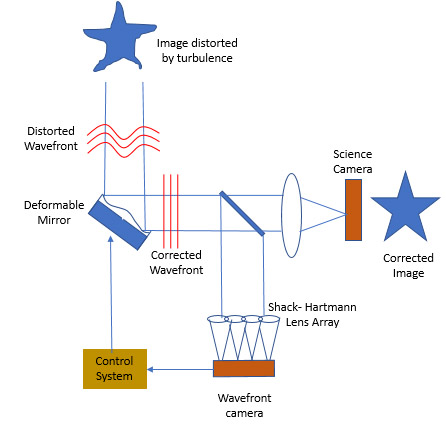
\includegraphics[width=0.4\textwidth]{immagini/ottiche-adattive.jpg}
\caption{Principio di funzionamento delle ottiche adattive. Un fronte d’onda distorto incide su uno specchio deformabile (con pistoni idraulici che si allungano o contraggono), la luce viene mandata a un sistema (waveform camera) che controlla se l’immagine della stella è soggetta a turbolenza oppure no, se è distorta (ovvero soggetta a turbolenza), i pistoncini idraulici deformano lo specchio iniziale per annullare l'effetto.}
\label{fig:ottiche-adattive}
\end{figure}

Per calcolare la deformazione da applicare alla lente per correggere il problema del seeing, si utilizza una \emph{stella guida}, che deve essere una stella molto brillante. Siccome non sempre è presente una stella molto brillante per effettuare la calibrazione, si utilizza una \emph{stella laser}, ovvero i telescopi sparano fasci laser brillanti che simulano la presenza di una stella brillante attraverso l'eccitazione di atomi di sodio a $\SI{90}{km}$ di altitudine. Un altro modo per evitare il seeing è banalmente evitare l'atmosfera terrestre, dunque utilizzando telescopi spaziali, che sono solamente diffraction-limited.

Si vuole, infine, sottolineare la differenza tra un telescopio e i suoi strumenti a bordo: ciascun telescopio, infatti, ha diversi strumenti a bordo. Questi si dividono in due categorie particolari: le \emph{photometric cameras}, utilizzate per l'imaging o la spettroscopia, e gli \emph{spettrografi}, utilizzati per la spettrografia, ovvero per misurare lo spettro della radiazione, che può essere in assorbimento o in emissione.